\documentclass[conference]{IEEEtran}
\usepackage{times}
% numbers option provides compact numerical references in the text. 
\usepackage[numbers]{natbib}
\usepackage{multicol}
\usepackage{tabularx}
\usepackage[bookmarks=true]{hyperref}
\usepackage{graphics} % for pdf, bitmapped graphics files
\usepackage{graphicx}
\usepackage[numbers]{natbib}
\usepackage{multicol}
\usepackage[bookmarks=true]{hyperref}
\usepackage{amsmath,amssymb,latexsym,float,epsfig,subfigure}
\usepackage{amsmath} % assumes amsmath package installed  % assumes amsmath package installed
\usepackage{mathtools, bbm}
\usepackage{lipsum}
\usepackage[export]{adjustbox}
\usepackage[normalem]{ulem} % underline
\usepackage{wrapfig}
\usepackage{multirow}
\usepackage{balance}
\usepackage{color}
\usepackage{url}
\usepackage{booktabs}
\usepackage{pifont}
\usepackage{algorithm, algorithmic}
\DeclareMathOperator*{\argmax}{argmax}
%\newcommand{\argmax}{\arg\!\max}
\newcommand{\norm}[1]{\left\lVert#1\right\rVert}
\def\bibfont{\footnotesize}
\pdfinfo{
	/Author (Deepak Gopinath, Brenna D. Argall)
	/Title  (Mode Switch Assistance to Human Intent Disambiguation)
	/CreationDate (January 31 2017)
	/Subject (Robots)
	/Keywords (Robots)
}
% numbers option provides compact numerical references in the text. 


\pdfinfo{
   /Author (Homer Simpson)
   /Title  (Robots: Our new overlords)
   /CreationDate (D:20101201120000)
   /Subject (Robots)
   /Keywords (Robots;Overlords)
}

\begin{document}

% paper title
\title{Information Theoretic Formulation of Intent Disambiguation}
\author{Author Names Omitted for Anonymous Review.}
% You will get a Paper-ID when submitting a pdf file to the conference system
%\author{Deepak Gopinath and Brenna D. Argall}

%\author{\authorblockN{Deepak Gopinath}
%\authorblockA{Department of Mechanical\\Engineering,
%Northwestern University\\
%Evanston, Illinois 30332\\
%Email: deepakedakkattilgopinath2015\\@u.northwestern.edu}
%\and
%\authorblockN{Brenna D. Argall}
%\authorblockA{Department of Mechanical\\Engineering,
%		Northwestern University\\
%		Evanston, Illinois 30332\\
%		Email: brenna.argall@northwestern.edu}
%	}

%\author{Deepak Gopinath$^{1}$ and Brenna D. Argall$^{2}$
%	\thanks{Manuscript received: March, 1, 2016; Revised June,
%		7, 2016; Accepted June, 29, 2016.}
%}
% avoiding spaces at the end of the author lines is not a problem with
% conference papers because we don't use \thanks or \IEEEmembership


% for over three affiliations, or if they all won't fit within the width
% of the page, use this alternative format:
% 
%\author{\authorblockN{Deepak E. Gopinath\authorrefmark{1}\authorrefmark{2},
%		Brenna D. Argall\authorrefmark{1}\authorrefmark{2}\authorrefmark{3}\authorrefmark{4}
%	}
%	\authorblockA{
%		\authorrefmark{1}Department of Mechanical Engineering, Northwestern University, Evanston, IL}
%	
%	\authorblockA{\authorrefmark{2}Rehabilitation Institute of Chicago, Chicago, IL}
%	
%	\authorblockA{\authorrefmark{3}Department of Physical Medicine and Rehabilitation, Northwestern University, Chicago, IL}
%	
%	\authorblockA{\authorrefmark{4}Department of Electrical Engineering and Computer Science, Northwestern University, Evanston, IL}
%	
%	\authorblockA{{\tt\small deepakgopinath@u.northwestern.edu}}
%	\authorblockA{{\tt\small brenna.argall@northwestern.edu}}
%}

\maketitle

\begin{abstract}
The effectiveness of assistive robots is closely related to their ability to infer the users' needs and intentions \textit{unambiguously} and provide appropriate assistance quickly and accurately. In this paper, we formulate the problem of intent disambiguation in information theoretic terms.  We propose two different methods for intent disambiguation using the information theoretic concepts of \textit{entropy} and \textit{KL divergence}. The proposed algorithms characterize the disambiguation capabilities of the system by the forward projection of probability distributions over goals utilizing an intent inference scheme and a kinematics model and computing the average information gain and content. Previous studies have shown that the success of a disambiguation algorithm depends on a variety of factors and parameters. To thoroughly investigate the impact of these various components, we present results from an extensive simulation-based study for point-like robots and a simulated robotic arm. Our results indicate that, compared to a baseline, the proposed disambiguation algorithms allow the robot to assist earlier during task execution. Additionally, we find that goal inference is more accurate and the total amount of assistance provided is higher.
\end{abstract}

\IEEEpeerreviewmaketitle

\section{Introduction}
Assistive machines such as robotic arms, smart wheelchairs  and myoelectric prosthesis have the potential to transform the lives of millions of people with motor impairments as a result injuries to the central nervous system~\citep{laplante1992assistive}. These machines can promote independence, enhance the quality of lives and revolutionize the way people interact with society. They can also help extend the mobility and manipulation capabilities of individuals thereby helping motor-impaired people perform activities of daily living in a more effective manner. 

An assistive robotic machine is typically controlled using a control interface such as a joystick, a switch-based head array or a sip-and-puff. These interfaces are low-dimensional, low-bandwidth and occasionally discrete. For this reason, they can often only operate in a subset of the entire control space. These subsets are referred to as \textit{control modes}. The efficacy of assistive machines rely on their ability to infer the users' needs and intentions and is often a bottleneck for providing appropriate assistance quickly, confidently and accurately. Due to the dimensionality mismatch between the high-dimensional robots and the low-dimensional interfaces, users are constrained to produce control commands that likely do not reveal their true intent. That is, the control interfaces act like filters that restrict the amount of information regarding the user's intent that gets passed through. 
%Furthermore, sparsity and noise in the control commands make the inference process even harder prompting the need for robust intent inference formalisms. 
In the context of assistive robotic manipulation, the first step of a task is often to reach for, and grasp, discrete objects in the environment. Therefore, \textit{intent inference} can be cast as a problem of computing the probability distributions over all possible discrete goals (objects) in the workspace. To estimate the most probable goal, intent inference mechanisms typically rely on various environmental cues and task-relevant features such as the robot and goal positions, human control commands and biometric measures. In contrast, our system infers intent primarily based on the information contained in the constrained control commands issued to the assistive machine. This approach is more cost effective and more likely to be accepted by the users. 

Our insight is that, at any given time, there is a specific set of control modes that are more informative \textit{for} the robot than others.  Therefore, by having the human provide input in these modes, the robot can possibly infer the human's underlying intent unambiguously. This, in turn, allows the robot to \textit{help assist the human achieve their desired goal earlier}.  This is important, because when the intent inference mechanism infers the incorrect goal (or is simply too slow), the user and autonomy often end up competing instead of collaborating. This can likely result lower user satisfaction often with significantly worse performance then either the human or robot could produce on their own.  In this paper, we address this problem by utilizing our characterization of control modes to develop a mode switch assistance paradigm that selects the control mode in which a user-initiated motion will \textit{maximally disambiguate} their intent.  To formulate the problem of \textit{intent disambiguation}, we use information theoretic notions of entropy and Kullback-Leibler (KL) divergence to characterize and quantify the intent disambiguation capabilities of each control mode.

%Our insight is that the information contained in control commands issued by the human when operating in certain control modes will be more useful \textit{for} the robot to perform intent inference more accurately. This in turn, will clarify the human's underlying intent unambiguously and help the robot to appropriately select the necessary kinds of assistance more effectively. In this paper, we formulate the problem of intent disambiguation in information-theoretic terms. Specifically, we rely on information theoretic notions of \textit{entropy} and \textit{Kullback-Leibler divergence} (KL divergence) to characterize and quantify the intent disambiguation capabilities of a control mode. We utilize this characterization of control modes to develop a mode switch assistance paradigm that selects the control mode in which a user-initiated motion will \textit{maximally disambiguate} their intent. 
%The disambiguation system will likely elicit more \textit{intent expressive} commands from the user by placing the user control in certain control modes.

In Section~\ref{sec:related_work} we present an overview of relevant research. Section~\ref{sec:math} presents set theoretic treatment of control modes followed by intent disambiguation and intent inference in Section~\ref{sec:disamb}. The study design and experimental methods are discussed in Section~\ref{sec:ed} followed by results in Section~\ref{sec:results}. Discussion and conclusions are presented in Sections~\ref{sec:discussions} and~\ref{sec:conclusions} respectively. 


\section{Related Work}\label{sec:related_work}
This section presents an overview of related works in information acquisition in robotics, intent inference in human-robot interaction and robot assistance for modal control. 
%
%Shared-autonomy in assistive machines aims to reduce the human's physical and cognitive burden during task execution without having the user completely cede manual control~\citep{philips2007adaptive, demeester2008user}. Some of the common shared-autonomy approaches include (a) hierarchical paradigms in which the higher level goals are entrusted with the user and the autonomy generates low-level control~\citep{kim2012autonomy}, (b) control allocation in distinct partitions of the control space~\citep{driessen2005collaborative} and (c) blending user controls and robot autonomy commands~\citep{muelling2017autonomy}. 

Information theoretic approaches are widely utilized in the field of machine learning and robotics for optimal experiment design, for efficient data collection processes and for informing search strategies. Robot assistance schemes that seek to elicit more informative cues \textit{from} the human to clarify the underlying intent can be thought of as an information acquisition problem. Intent acquisition can leverage the underlying synergies and shared intentionality~\citep{tomasello2007shared} of human-robot teams and can be an active process in which the robot performs actions (for example, selecting a control mode or executing a robot motion) that will nudge the human to reveal her/his intent more clearly~\cite{sadigh2016information, sadigh2016planning}. Information theoretic metrics such as a KL divergence can be utilized to identify regions of the sample space that will maximize information gain~\citep{tong2001active} and subsequently guide the data sampling process. Sensing robots designed for automated exploration and data acquisition tasks can benefit from exploring more information-rich regions in the environment~\citep{atanasov2014information}. If the spatial distribution of information density is known \textit{a priori}, information maximization can be accomplished by maximizing the ergodicity of the robot's trajectory with respect to the underlying information density map~\citep{miller2013trajectory, miller2016ergodic}. 

For an assistive machine to provide appropriate kinds of assistance accurately and at the right time, it needs to have a good estimate of the human's underlying intent. Intent inference algorithms, therefore, play a vital role in the success of a assistive system. Intent inference and recognition can be classified into two broad categories: heuristic approaches and model-based approaches. Heuristic approaches are often simpler and computationally light-weight and seek to find direct mappings between various task relevant features (such as motion cues) and the human's underlying intention~\citep{baker2007goal, baker2009action}. On the other hand, in model-based approaches the system maintains a model of how a human maps states to control actions. The model can either be learned from data or can be hand-designed based on domain knowledge. For example, the human can be modeled within the Partially Observable Markov Decision Process (POMDP)~\citep{dragan2013policy, taha2011pomdp} framework and is assumed to behave according to a control policy that maps states to actions. However, in model-based approaches incorporating the entire history of states requires estimation of joint probability distributions over past states which can become computationally expensive and intractable quickly.

When there is a mismatch between the dimensionality of the problem and the control interface users have to continuously shift their focus from the task at hand to the choice of control mode during task execution, thereby resulting in a higher cognitive load. To solve this problem, various mode switching assistance paradigms have been proposed to alleviate task effort. For example, an automatic time-optimal mode switch assistance has been proposed which has shown to significantly improve user satisfaction~\citep{herlant2016assistive}. In the area of myoelectric prosthetics, dynamic switching approaches that learn the most effective control option during task execution using temporal difference and reinforcement learning have also been proposed~\cite{pilarski2012dynamic}. 


\section{Mathematical Notation}\label{sec:math}
This section describes the mathematical notation used in our intent disambiguation algorithm that computes a control mode that maximally disambiguates between the various goals.
We develop this algorithm specifically for robotic manipulation scenarios in which the user is controlling a robotic arm to reach for and interact with various discrete objects in the environment.

% Section~\ref{ssec:notation} outlines the mathematical notation used in this paper. Section~\ref{ssec:set_modes} presents a set-theoretic treatment of control modes and Section~\ref{ssec:disamb} describes the disambiguation algorithm. The mathematical details of the intent inference paradigms are outlined in detail in Section~\ref{ssec:inference}.
\subsection{Probability Distribution Over Goals}\label{ssec:notation}
 In assistive robotic manipulation, intent inference is most commonly process of estimating the user's intended goal out of a set of discrete objects in the environment~\citep{calli2015ycb}. The set of all candidate goals is denoted by $\mathcal{G}$ with $n_g = \vert\mathcal{G}\vert$ and let $g^i$ refer to the $i^{th}$ goal with $i \in [1,2,\dots, n_g]$. At any time $t$, the likelihood of goal $g$ being the desired goal follows a categorical probability distribution whose sample space is $\mathcal{G}$. 
 That is, 
 \begin{equation*}
 g \sim \textbf{Cat}(n_g | \boldsymbol{p}(t)) = \prod_{i=1}^{n_g}p^{i}(t)^{[g = g^i]}
 \end{equation*}
where, $[g = g^i]$ is the Iverson bracket and evaluates to 1 if $g = g^i$, 0 otherwise. $\boldsymbol{p}(t)$ denotes the probability distribution over goals such that $\boldsymbol{p}(t) = [p^1(t), p^2(t),\dots, p^{n_g}(t)]^{T}$ where $p^i(t)$ denotes the probability associated with goal $g^i$.  The probability $p^i(t)$ represent the robot's \textit{confidence} that goal $g^i$ is the human's intended goal. 


\subsection{Set Theoretic Treatment of Control Modes}\label{ssec:set_modes}
%
%The limitations of the control interfaces necessitate the control space $\mathcal{K}$ to be partitioned into control modes. Let $\mathcal{M}$ denote the set of all control modes with $n_m = \vert\mathcal{M}\vert$. Additionally, let $m^i$ refer to the $i^{th}$ control mode where $i \in [1,2,\dots,n_m]$. Each control mode $m^i$ is a subset of $\mathcal{K}$ such that $\bigcup\limits_{i=1}^{n_m} m^i$ spans all of the controllable dimensions.\footnote{Note that a dimension $k \in \mathcal{K}$ can be an element of multiple control modes.} Let $\boldsymbol{e}^i$ be the standard basis vectors that denote the unit velocity vector along the $i^{th}$ control dimension.\footnote{For the rotational control dimensions, the velocity is specified with respect to the end-effector of the robotic frame.} Furthermore, the user can only operate in one of the $n_m$ control modes at any given time $t$. Therefore, the user can only access smaller subsets of $\mathbb{R}^{n_k}$ via the control interface with $\mathcal{U}_{m^i}$ denoting the subset of $\mathbb{R}^{n_k}$ accessible from control mode $m^i$. Figure 1 represents this in a pictorial fashion for a robot residing in $\mathbb{R}^2$. 
The low dimensionality of the control interfaces necessitates the control space to be partitioned into control modes.
Let $\mathcal{K}$ be the set of all controllable dimensions of the robot and $k^i$ represent the $i^{th}$ control dimension where $i \in [1,2,\dots,n_k]$ with $n_k = \vert\mathcal{K}\vert$. the number of controllable dimensions ($n_k$) depends on the robotic platform; for example, a 2D point robot that operates in $\mathbb{R}^2$ has $n_k = 2$ whereas $n_k =6$ for a 6DoF robotic manipulator. 
%Lastly, let $\boldsymbol{u_h} \in \mathbb{R}^{n_k}$ denotes the human control command issued via the control interface and $\boldsymbol{u_r} \in \mathbb{R}^{n_k}$ denote the robot autonomy command.

 Let $\mathcal{M}$ denote the set of all control modes with $n_m = \vert\mathcal{M}\vert$. Additionally, let $m^i$ refer to the $i^{th}$ control mode where $i \in [1,2,\dots,n_m]$. Each control mode $m^i$ is a subset of $\mathcal{K}$ such that $\bigcup\limits_{i=1}^{n_m} m^i = \mathcal{K}$. The cardinality of each mode denoted by $\vert m \vert$ indicates the number of dimensions that can be controlled when operating in $m$.\footnote{Note that a dimension $k \in \mathcal{K}$ can be an element of multiple control modes.} Furthermore, the user can only operate in one of the $n_m$ control modes at any given time $t$. That is, for each $m \in \mathcal{M}$, the subspace of $\mathcal{R}^{n_k}$ that is accessible corresponds to $\mathcal{R}^{\vert m \vert}$ whose orthonormal basis vectors are given by $\boldsymbol{e}^k \;\; \forall \;\; k \in m$. Maximum velocity limits along each dimension imposes further constraints on the set of control commands that are available in each mode. The set of control commands denoted by $\mathcal{U}^m$, can be written as 
\begin{equation*}
\mathcal{U}^m = \{\boldsymbol{u} | \boldsymbol{u} \in \mathcal{R}^{\vert m \vert} ~ and ~ \norm{\boldsymbol{u}}_{\infty} \leq c \} 
\end{equation*}
where $c$ denotes the maximum velocity along any dimension $k$ and $\norm{\cdot}_{\infty}$ denotes the $L_\infty$ norm. 
%Therefore, the set $\mathcal{U}^m$ corresponds to a hypercube of dimensionality $\vert m \vert$ embedded in $\mathcal{R}^{n_k}$. In other words $\mathcal{U}^m$ is a $\vert m \vert$-cube with edge length equals $2c$. Without loss of generality, the velocity limits can be different for different control dimensions in which case $\mathcal{U}^m$ will correspond to a hypercuboid. Figure 1 represents this in a pictorial fashion for $\mathbb{R}^2$. 
% \begin{figure}[h]
%	\centering
%	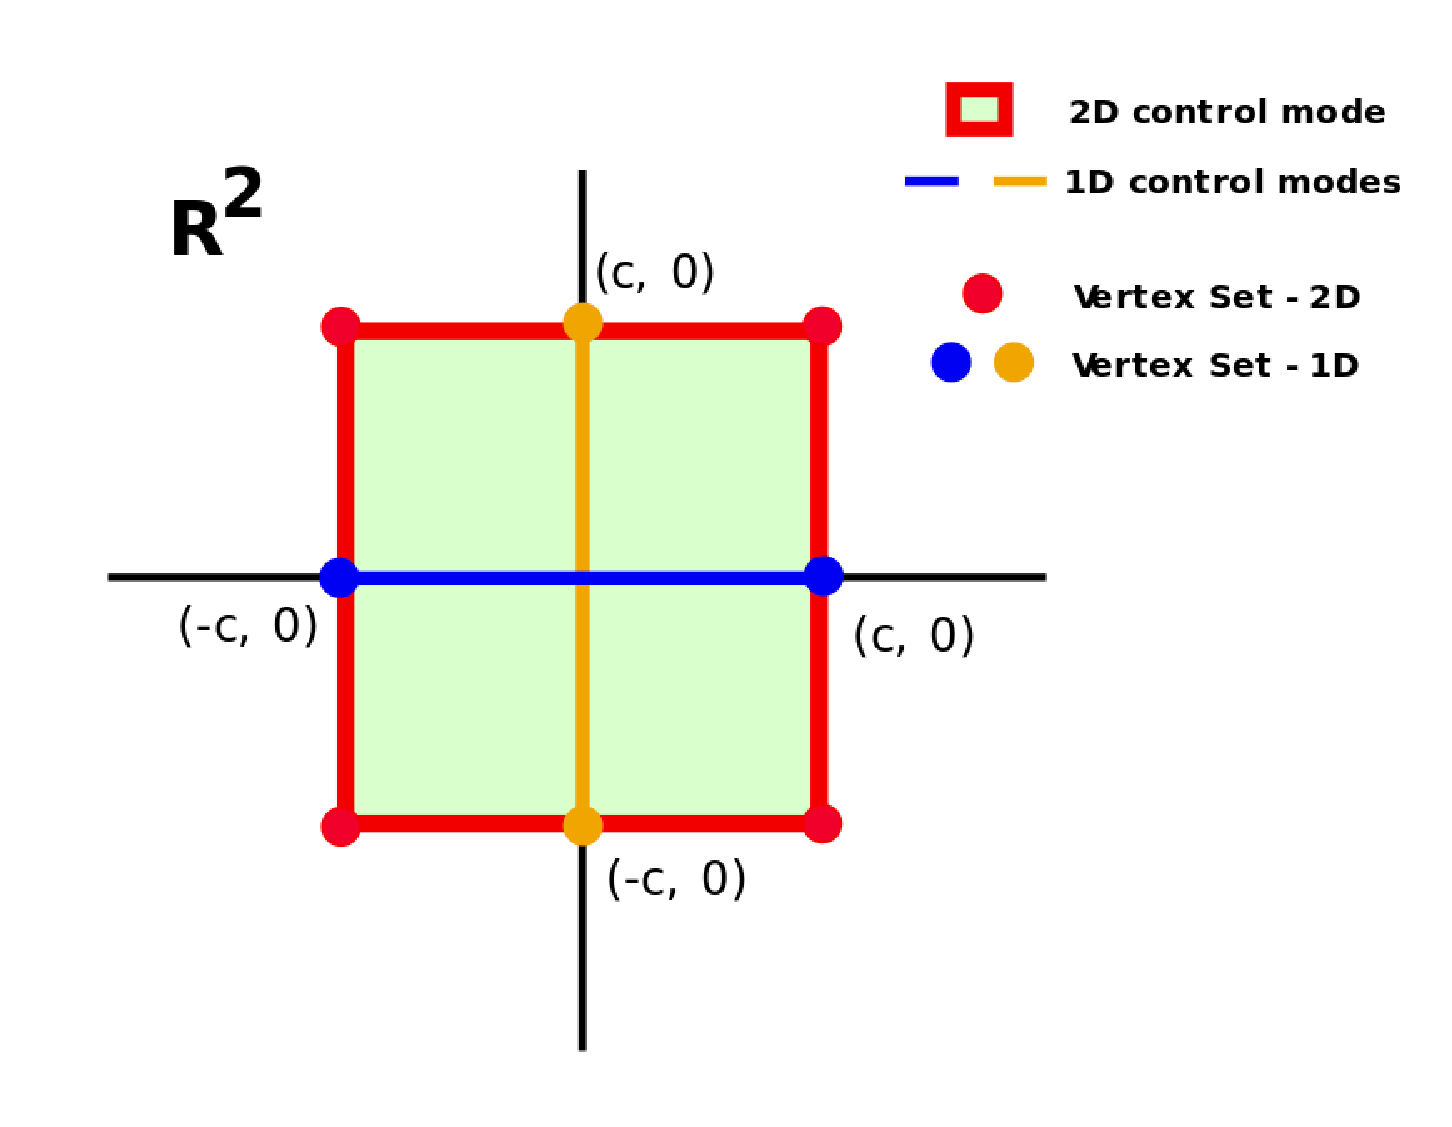
\includegraphics[width= 0.8\hsize, height=0.2\vsize]{./figures/R2_ControlModes.eps}
%	\vspace{-0.35cm}
%	\caption{Illustration of 1D and 2D control modes in a two-dimensional control space, $\mathbb{R}^2$. Note that this space can be embedded in a higher dimensional space such as $\mathbb{R}^3$, $\mathbb{SE}(2)$ and $\mathbb{SE}(3)$. The 1D control modes are shown in blue and orange and the 2D control mode is shown as the green shaded area within the red square. The vertex set denotes the maximum magnitude control commands that can be issued when operating in a control mode. }
%	\label{fig:r2_modes}
%\end{figure}

% The disambiguation formalism developed in Section~\ref{ssec:disamb} is agnostic to the particular form of intent inference. However, the algorithm assumes that $\boldsymbol{p}(t)$ can be forward projected in time by iteratively applying the intent inference algorithm. 
\section{Intent Disambiguation}\label{sec:disamb}

This section describes our two proposed approaches for intent disambiguation using information theoretic concepts and the different intent inference schemes that work in conjunction with the disambiguation algorithms. 

\subsection{Need For Intent Disambiguation}

Our aim is to develop a metric that will capture the ``disambiguation capability'' of a control dimension/mode. Subsequent user operation of the robot in the control mode with maximum disambiguation capability will likely ``help'' the robot to perform better intent inference and may result in the robot providing appropriate kinds of assistance.

At any given time $t$, the probability distributions over goals encodes the human's underlying intent. The time evolution of the probability distribution, however, depends on the choice of the intent inference scheme and the various task relevant features and parameters that contribute to it. If the evolution is sensitive to the user control command (denoted by $\boldsymbol{u_h}$) then it is likely that the goal probabilities evolve differently as the user operates the robot in different control modes. User generated motion along certain control dimensions may reveal the human's intent with less ambiguity. That is, intent disambiguation serves as a mechanism that will enhance the accuracy of intent inference. Various types of intent inference schemes used in conjunction with the proposed disambiguation algorithms in our paper are described in detail in Section~\ref{ssec:inference}. 


\subsection{Forward Projection of $\boldsymbol{p}(t)$}
The first step towards the computation of the disambiguation metric $D_m$ for each $m \in \mathcal{M}$ is the forward projection of the probability distribution $\boldsymbol{p}(t)$ from current time $t_a$ to $t_b$ such that $t_a < t_b$. The exact computation of the projected probability distribution will depend on the underlying intent inference computation---for example, whether it depends on the robot position ($\boldsymbol{x_r}$), which can be computed from the human control command (denoted by $\boldsymbol{u}_h$) applied to the robot kinematics model or $\boldsymbol{u}_h$. All parameters and features which affect the computation of $\boldsymbol{p}(t)$ are denoted as $\boldsymbol{\Theta}$. If the inference mechanism depend on the control command, the projected probability distribution at time $t_b$ given by $\boldsymbol{p}(t_b)$ depends on $\boldsymbol{u_h}$. For the purposes of computation of the disambiguation metric, in each mode $m \in \mathcal{M}$, we only consider a subset of control commands from $\mathcal{U}^m$, and is denoted by $Vert(\mathcal{U}^m)$. The set $Vert(\mathcal{U}^m)$ is given by
\begin{equation*}
Vert(\mathcal{U}^m) = \{\boldsymbol{u} \in \mathcal{U}^m ~|~ \boldsymbol{u} = \argmax_{\boldsymbol{u} \in \mathcal{U}^m} \norm{\boldsymbol{u}}_{2}\}
\end{equation*}
where $\norm{\cdot}_2$ is the Euclidean norm.\footnote{$Vert(\mathcal{U}^m)$ corresponds to the ``vertices'' of the $|m|$-dimensional hypercube that is the space of control commands accessible from mode $m$.} 

The probabilities are forward projected for each of the possible control commands available in $Vert(\mathcal{U}^m)$ and a weighted average of the disambiguation metric computations on each of the projected probabilities is used to characterize the control mode $m$ (Algorithm~\ref{alg:disamb}, Lines 3-11). In the following sub-sections we present two different methods to compute the disambiguation metric for a given mode $m$. 

 \begin{figure}[h]
	\centering
	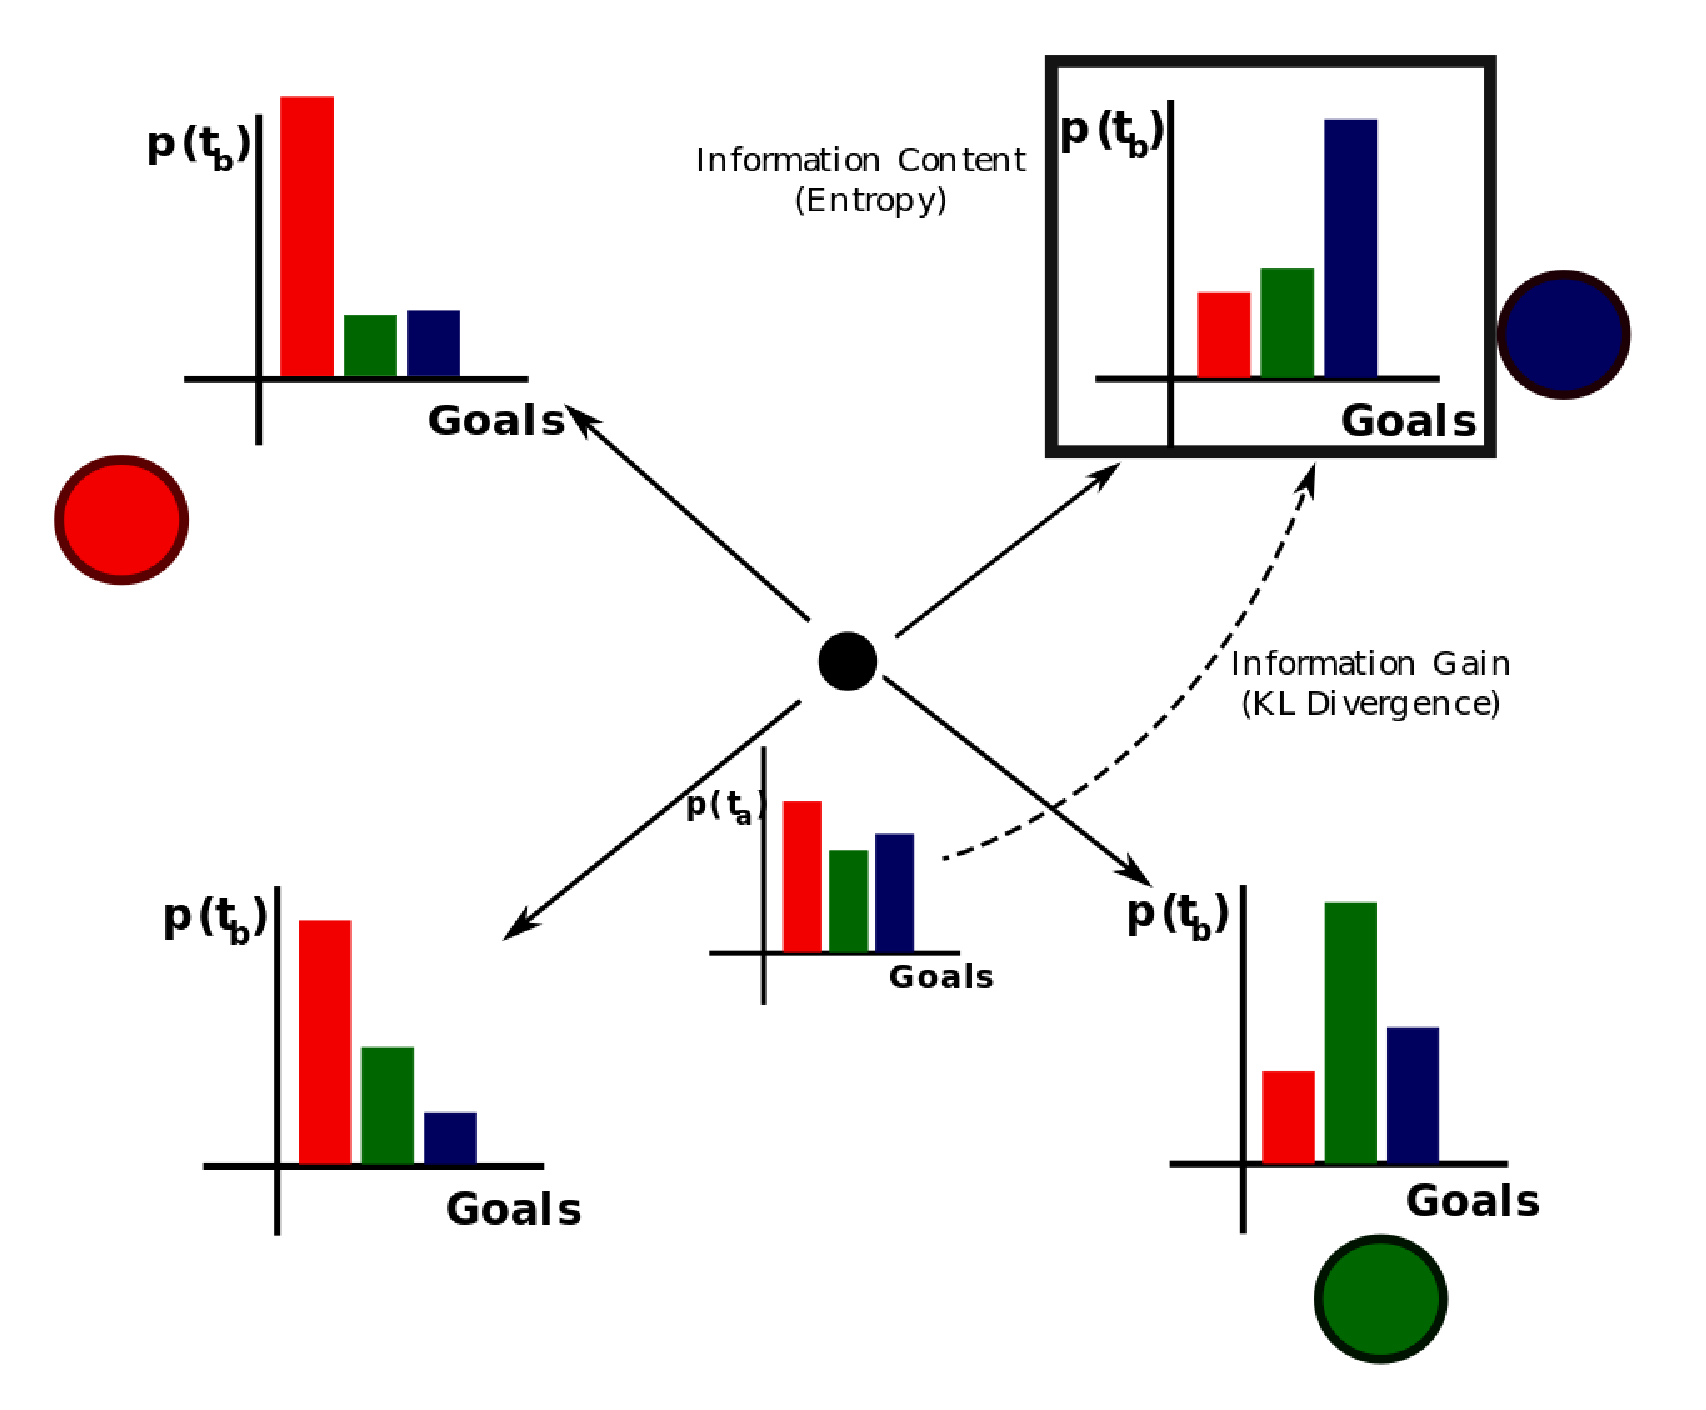
\includegraphics[width= 1.\hsize, height=0.3\vsize]{./figures/Disamb_Compute.eps}
	\vspace{-0.35cm}
	\caption{Illustration of computation of $D_m$ in $\mathbb{R}^2$. The goals are shown in red, green and blue and the robot in black. The probability distributions are forward projected for all $\boldsymbol{u_h} \in Vert(\mathcal{U}^m)$. The change in the overall shape of the probability distribution upon evolving from $\boldsymbol{p}(t_a)$ to $\boldsymbol{p}(t_b)$ amounts to the information \textit{gain} and is captured by the \textit{KL divergence}. The entropy of $\boldsymbol{p}(t_b)$ captures the information \textit{content} in the projected distribution.} 
	\label{fig:disamb_compute}
\end{figure}


\subsection{Entropy Based Disambiguation Metric}\label{sssec:ent}
The entropy of the probability distribution captures the average information content of a stochastic source of data. Lower entropy indicates higher certainty in the value of the random variable and vice-versa. Therefore, in the context of intent disambiguation entropy of the projected probability distribution, $\boldsymbol{p}(t_b)$, can be used as a measure of how confident the system is in its prediction of human intent. That is, entropy can be used a measure of disambiguation. Lower the entropy better the disambiguation due to higher certainty in the human's intended goal. For a discrete random variable $X$ with possible values $\{x_1, x_2,\dots x_n\}$, the Shannon entropy is defined as 
\begin{equation*}
ENT(P(X)) = -\sum_{i = 1}^{n} P(x_i)log_{2}P(x_i)
\end{equation*}
where $P(X)$ denotes the probability mass function.
The disambiguation capability of a control mode $m$ is characterized by computing a weighted average of the entropies of projected probability distributions for all possible control commands $\boldsymbol{u_h} \in Vert(\mathcal{U}^m)$.
That is
\begin{equation}
D_m = \frac{1}{\vert Vert(\mathcal{U}^m) \vert}\sum_{\boldsymbol{u_h} \in Vert(\mathcal{U}^m)}  ENT(\boldsymbol{p}(t_b; \boldsymbol{u_h}))
\end{equation}
where $\boldsymbol{p}(t_b; \boldsymbol{u_h})$ denotes the projected probability distribution at time $t_b$ when the control command used for forward projection is $\boldsymbol{u_h}$.
\subsection{KL divergence Based Metric}\label{sssec:kl}
Although entropy can capture information \textit{content}, intent disambiguation can likely benefit from the quantification of the information \textit{gain} regarding the human's intended goal as a result of user-initiated motion in a control mode $m$. 
KL divergence, also known as relative entropy, measures how one probability distribution differs from another distribution. KL divergence is widely used in the context of Bayesian inference to compute the information gain when the prior is updated to the posterior in the light of new evidence. In the context of disambiguation we can treat the projected probability distribution as the posterior and distribution at time $t_a$ to be the prior. KL divergence can then be used to characterize the \textit{information gain} regarding the human's intended goal as a result of the application of $\boldsymbol{u_h}$.
For a discrete random variable $X$ with possible values $\{x_1, x_2,\dots x_n\}$ the KL divergence is defined by
\begin{equation*}
KL(P||Q) = -\sum_{i=1}^{n}P(x_i)log_2\frac{Q(x_i)}{P(x_i)}
\end{equation*}
where $P(X)$ and $Q(X)$ are two different probability mass distributions. 
  More specifically, the disambiguation capability of control mode $m$ is computed by averaging the information gain for all possible control commands $\boldsymbol{u_h} \in Vert(\mathcal{U}^m)$. That is the disambiguation metric can be computed as 
\begin{equation*}
D_m = \frac{1}{\vert Vert(\mathcal{U}^m) \vert}\sum_{\boldsymbol{u_h} \in Vert(\mathcal{U}^m)} KL(\boldsymbol{p}(t_b; \boldsymbol{u_h})||\boldsymbol{p}(t_a))~~~~.
\end{equation*}
\begin{algorithm}[t]
	\caption{Calculate $\boldsymbol{p}(t_b)$, $D_m$}
	\label{alg:disamb}
	\begin{algorithmic}[1]
		\REQUIRE $\boldsymbol{p}(t_a), \boldsymbol{x}_r(t_a), \Delta t, t_a < t_b, \boldsymbol{\Theta}$
		\FOR{$m=1\dots n_m$}
		\STATE Initialize $D_m = 0$
		
		\FOR{$\boldsymbol{u_h} \in Vert(\mathcal{U}^m)$}
		\STATE Initialize $t = t_a, \boldsymbol{x_r}(t) = \boldsymbol{x_r}(t_a), \boldsymbol{p}(t) = \boldsymbol{p}(t_a)$
		\WHILE{$t \leq t_b$}
		\STATE $\boldsymbol{p}(t + \Delta t) \leftarrow \text{UpdateIntent}(\boldsymbol{p}(t), \boldsymbol{u}_h; \boldsymbol{\Theta})$
		\STATE $\boldsymbol{x}_r(t + \Delta t) \leftarrow \text{SimulateKinematics}(\boldsymbol{x}_r(t), \boldsymbol{u}_h)$
		\STATE $t \leftarrow t + \Delta t$
		\ENDWHILE
		
		\STATE $D_m \leftarrow D_m + \frac{1}{\vert Vert(\mathcal{U}^m) \vert} ENT(\boldsymbol{p}(t_b)) $
		
		or
		
		\STATE $D_m \leftarrow D_m + \frac{1}{\vert Vert(\mathcal{U}^m) \vert} KL(\boldsymbol{p}(t_b) \vert\vert \boldsymbol{p}(t_a)) $
		
		\ENDFOR
		\ENDFOR
	\end{algorithmic}
\end{algorithm}
The control mode with highest disambiguation capability $m^*$ is given by $\argmax_m D_m$. Disambiguation mode $m^*$ is the control mode that system chooses \textit{for} the human to better estimate their intent. Any control command issued by the human when operating in $m^*$ is likely to be more beneficial for the robot to determine the human's intended goal. 

\subsection{Intent inference}\label{ssec:inference}
  The disambiguation power of our algorithm is closely linked to the inference power of different choices of inference mechanisms. The update rule for the probability distribution over goals is determined by the choice of inference schemes (Algorithm~\ref{alg:disamb}, Line 6) as a result of which the projected probability distributions, $\boldsymbol{p}(t_b)$ and the disambiguation metric $D_m$, likely are going to be different. This section describes the different types of intent inference schemes that work in conjunction with the disambiguation algorithms proposed in Section~\ref{sec:disamb}.
%This is because, during the forward projection step, different intent update schemes result in different projections and affects the computation of the disambiguation metric. 

\subsubsection{Heuristic Approaches}
Heuristic approaches based on \textit{confidence} functions~\citep{dragan2013policy} seek to find direct mappings between instantaneous cues and underlying human intentions. For every goal $g \in \mathcal{G}$, the system maintains an associated set of confidences denoted by $\mathcal{C}$. The system designer has the freedom to choose the set of features that will inform the confidence functions. For example, a simple proximity-based confidence function used extensively in literature is
\begin{equation}
c(\boldsymbol{x_r}, \boldsymbol{x_g}) = max\Big(0, 1 - \frac{\norm{\boldsymbol{x_r} - \boldsymbol{x_g}}}{r}\Big)
\end{equation}
where $\boldsymbol{x_r}$ is the robot position, $\boldsymbol{x_g}$ is the goal position, $r$ is the radius beyond which the confidence function is always 0 and $\norm{\cdot}$ is an appropriate distance metric. 
A slightly more information-rich variant that aims to capture the ``directedness'' of the human control command to a particular goal position is
\begin{equation*}
c({\boldsymbol{x_r},\boldsymbol{x_g}, \boldsymbol{u}_{h}}) = \boldsymbol{u}_h\cdot(\boldsymbol{x}_{g} - \boldsymbol{x_r})
\end{equation*}
where $\boldsymbol{u_h}$ is the human control command. These confidence functions rely on instantaneous features and therefore are amnesic and can exhibit chatter behavior~\citep{dragan2012formalizing}.

%One of the drawbacks of heuristic approaches is that information contained in the history of states is typically ignored. As a result, the inference is not robust to external noise and can exhibit chatter behavior. 
\subsubsection{Bayesian Approaches}
Bayesian approaches to intent inference consists of iteratively updating of the belief (probability distribution over goals) as new evidence arrives at every time-step. The Bayesian update equation for the probability distribution over goals is given by
\begin{equation*}
\underbrace{p(g_t| \boldsymbol{u}^{1:t}_{\boldsymbol{h}}, \boldsymbol{\Theta})}_{posterior} = \eta \underbrace{p(\boldsymbol{u}^{1:t}_{\boldsymbol{h}} | g_t, \boldsymbol{\Theta})}_{likelihood}\underbrace{p(g_{t-1})}_{prior}
\end{equation*}
where $\eta$ is the normalization factor, $\boldsymbol{u}^{1:t}_{\boldsymbol{h}}$ is the entire history of control commands and $\boldsymbol{\Theta}$ denoted all other task-relevant and environment features that informs the inference process. The likelihood function is related to how the human teleoperates the robot in order to accomplish a goal and can be either learned from data, or be hand-designed utilizing domain knowledge. Under first-order Markovian assumption the equation can be simplified by only considering the control command at the current time step $t$. 
\subsubsection{Dynamic Neural Field Based Approaches}
Dynamic neural fields are differential equations in time that governs the time evolution of dynamical state variables, with some specific properties such as recurrent interactions between the state variables, robustness to external noise and memory. Dynamic neural fields were originally conceived to explain cortical population neuronal dynamics, based on the hypothesis that the excitatory and inhibitory neural interactions between local neuronal pools form the basis of cortical information processing~\citep{schoner2008dynamical, schoner1995dynamics}. 
When applied to the problem of intent inference, the individual goal probabilities are treated as constrained dynamical state variables whose time evolution is determined by a dynamic neural field such that $p^i(t) \in [0, 1]$ and $\Sigma_{1}^{n_g}p^{i}(t) = 1$~\citep{gopinath2017disamb}. 
%Recurrent interactions between the state variables, robustness to external noise and inherent memory make dynamic neural fields an ideal candidate for an intent inference engine. 

% The dynamical system that governs the time evolution of goal probabilities can be generically written as 
%\begin{equation*}
%\dot{\boldsymbol{p}}(t) = F(\boldsymbol{p}(t), \boldsymbol{u}_h ; \boldsymbol{\Theta})
%\end{equation*}
%where $F$ represents the nonlinear vector field, $\boldsymbol{u}_h$ is the human control input and $\boldsymbol{\Theta}$ represents all other task-relevant features and parameters that affect the time-evolution of the probability distribution. 
The full specification of the neural field is given by
\begin{multline}\label{eq:dft}
\frac{\partial \boldsymbol{p}(t)}{\partial t} = \frac{1}{\tau}\bigg[-\mathbb{I}_{n_g\times n_g}\cdot\boldsymbol{p}(t) + \underbrace{\frac{1}{n_g}\cdot\mathbbm{1}_{n_g}\bigg]}_{\text{rest state}} + \\ \underbrace{\boldsymbol{\lambda}_{n_g\times n_g}\cdot\sigma(\boldsymbol{\xi}(\boldsymbol{u}_h;\boldsymbol{\Theta}))}_{\text{excitatory + inhibitory}}
\end{multline}
where time-scale parameter $\tau$ determines the memory capacity of the system, $\mathbb{I}_{n_g\times n_g}$ is the identity matrix, $\mathbbm{1}_{n_g}$ is a vector containing all ones of dimension $n_g \times 1$, $\boldsymbol{\lambda}$ is the control matrix that controls the excitatory and inhibitory aspects, $\boldsymbol{\xi}$ is a function that encodes the nonlinearity through which human control commands and task features affect the time evolution, $\boldsymbol{\Theta}$ represents all other task-relevant features and parameters that affect the time-evolution of the probability distribution, and $\sigma$ is a biased sigmoidal nonlinearity given by $\sigma(\boldsymbol{\xi}) = \frac{1}{1 + e^{-\boldsymbol{\xi}}} - 0.5$. 
%In the absence of any information or cues, the probability distribution settles to a resting state which is a uniform distribution, that is whenever $\boldsymbol{u}_h = 0$, $\boldsymbol{\xi} = \vec{0}$. 
Given the initial probability distribution at time $t_a$ Equation~\ref{eq:dft} can be solved numerically from $t \in [t_a, t_b]$ using a simple Euler algorithm with a fixed time-step $\Delta t$. The design of $\boldsymbol{\xi}$ is informed by what features of the human control input and environment capture the human's underlying intent most effectively. We rely on the \textit{directedness} of the human control commands towards a goal, the \textit{proximity} to a goal and the \textit{agreement} between the human commands and robot autonomy.

\section{Experimental Evaluation}\label{sec:ed}
We evaluate the efficacy of the proposed disambiguation algorithm on simulated point-like robots and a simulated robotic manipulator that operates in a \textit{shared-control} setting. This section describes the shared-control paradigm used in our experiments and the details of the simulation experiment protocol.
%In this section we describe our simulation experiments conducted on simulated point-like robots and a simulated robotic manipulator to evaluate the effectiveness of our disambiguation algorithm. 
\subsection{Shared Control}\label{ssec:shared-control}
Shared autonomy in assistive robotics aims to reduce the human's physical and cognitive burden during task execution without having the user to completely cede manual control. Some common shared-control approaches include (a) hierarchical paradigms in which the choice of a high-level goal is entrusted to the user and the autonomy generates low-level control~\citep{kim2012autonomy} and (b) signal-level paradigms in which the user and robot's control commands are blended together~\citep{muelling2017autonomy}. Shared control systems often require a good estimate of the human's intent to determine when and how to share control. Therefore, intent inference and disambiguation play a vital role in the seamless operation and success of a shared control system. In our experimental evaluation, control-sharing is achieved with a blending-based paradigm in which the final control command issued to the robot is a weighted linear combination of the user control command and robot autonomy.
\subsubsection{Robot Autonomy}\label{sssec:autonomy}
%The autonomous control policy generates control command
%$\boldsymbol{u}_r \leftarrow f_{r}(\boldsymbol{x})$
%where $f_{r}(\cdot) \in \mathcal{F}_{r}$, and $\mathcal{F}_{r}$ is the set of all control behaviors corresponding to different tasks. 
%Specifically, let $\boldsymbol{u}_{r,g}$ be the autonomy command associated with goal $g$. 

The robot control command $\boldsymbol{u}_{r,g}$ is generated using a simple potential field which is defined in all parts of the state space~\citep{khatib1986real}. Every goal $g$ is associated with a potential field $\gamma_g$ which treats $g$ as an attractor and all the other goals in the scene as repellers. That is,
\begin{equation*}
\dot{\boldsymbol{x}}_r^{attract} = \boldsymbol{x}_{g} - \boldsymbol{x_r}
\end{equation*}
 where $\dot{\boldsymbol{x}}_r$ indicates the velocity of the robot, $\boldsymbol{x}_{g}$ is the location of goal $g$. Each dimension of $\dot{\boldsymbol{x}}_r^{attract}$ can be interpreted as the magnitude of the \textit{attractive pull} towards the goal along that dimension. 
The repeller velocity is given by
\begin{equation*}
\dot{\boldsymbol{x}}_r^{repel} = \sum_{i \in \mathcal{G} \setminus g} \frac{\boldsymbol{x_r} - \boldsymbol{x}_{g^i}}{\mu(\norm{\boldsymbol{x_r} - \boldsymbol{x}_{g^i}}^2)}
\end{equation*}
 $\mu$ controls the magnitude of the repeller velocity. The autonomy command $\boldsymbol{u}_{r,g}$ is computed as a summation of the attractor and repeller velocities.
%\begin{equation*}
%\boldsymbol{u}_{r,g} = \dot{\boldsymbol{x}}_r^{attract} + \dot{\boldsymbol{x}}_r^{repel} 
%\end{equation*}
%$\gamma_g$ operates in the full six dimensional Cartesian space, and treats position and orientation as independent potential fields. 
\subsubsection{Blending Paradigm}\label{sssec:blending}
The final control command $\boldsymbol{u_f}$ issued to the robot then is given by
\begin{equation*}
\boldsymbol{u_f} = \alpha\cdot \boldsymbol{u}_{r,g^*} + (1 - \alpha)\cdot \boldsymbol{u}_h
\end{equation*}
where $g^*$ is the most confident goal and corresponds to the mode of $\boldsymbol{p}(t)$. The blending parameter, $\alpha$ is a piecewise linear function of the $p(g^*)$ and is specified as
$$
\alpha = \left\{
\begin{array}{ll}
0 & \quad\quad~~~ p(g^*) \leq \rho_1 \\
\frac{\rho_3}{\rho_2 - \rho_1}\cdot p(g^*) &  \quad \text{if}\quad \rho_1 < p(g^*) \leq \rho_2  \\
\rho_3 & \quad\quad~~~ p(g^*) > \rho_2 	
\end{array}
\right.
$$
with $\rho_i \in [0, 1] \;\forall\; i \in [1,2,3]$ and $ \rho_2 > \rho_1$. 
In our implementation, we empirically set $\rho_1 = \frac{1.2}{n_g}, \rho_2 = \frac{1.4}{n_g}$ and $ \rho_3 = 0.7$.
\subsubsection{Baseline Mode Switch Assistance}\label{sssec:baseline}
As a baseline for the simulation experiments described in Section~\ref{sec:ed} we also propose a simple greedy mode switch assistance scheme. At any given time $t$, the system selects the control mode which has the \textit{maximum attractive pull} or \textit{maximum potential} towards the goal. For each control dimension $k$, the magnitude of the $k^{th}$ dimension of $\dot{\boldsymbol{x}}_r^{attract}$ is a measure of the attractive potential along $k$. Each control mode $m \in \mathcal{M}$ is summarized by the total attractive potential of all control dimensions $k \in m$.

\subsection{Point Robot Simulation Setup}
\subsubsection{Robot Workspace}
Our simulations were performed on point-like robots that reside in $\mathbb{R}^2$, $\mathbb{R}^3$, $\mathbb{SE}(2)$ and $\mathbb{SE}(3)$ spaces. The translational workspace limits were set at $[-0.4m, 0.4m]$ along each translational dimension and the orientation limits were set at $[0, 2\pi]$ along each rotational axis. Table~\ref{tbl:manip} lists all the factors there were randomized and manipulated for each trial. 
\begin{table}[t]
	\centering
	\begin{tabular}{|p{3cm}|p{3cm}|}
		\hline
		\textbf{Variable} &\textbf{Range}  \\ \hline
		$n_g$ &  $[2,6]$ \\ \hline
		$\mathcal{M}$ & Randomly selected from Table~\ref{tbl:cmp} conditioned on the space\\ \hline
		Intent Inference & [`Confidence', `Bayes', `DFT'] \\ \hline
		Initial Robot Position & Randomized within workspace limits \\ \hline
		Goal Positions & Randomized within workspace limits \\ \hline
		Intended Goal & Randomly chosen from $\mathcal{G}$ \\ \hline
	\end{tabular}
	\vspace{.2cm}
	\caption{Randomized Factors for Each Simulation Trial} 
	\label{tbl:manip}
	\vspace{-.5cm}
\end{table}

\subsubsection{Mode Switch Schemes}
Four different mode switching schemes were activated during each simulation trial, three of which performed intent disambiguation and one which served as a baseline for comparison. The disambiguation algorithms were entropy-based (Section~\ref{sssec:ent}), KL divergence based (Section~\ref{sssec:kl}) and a heuristic-based approach developed in an earlier work~\citep{gopinath2017mode}. We used the mode switching scheme described in Section~\ref{sssec:baseline} as the baseline for comparison. 
\subsubsection{Simulated $\boldsymbol{u_r}$ and $\boldsymbol{u_h}$}
The simulated robot autonomy $\boldsymbol{u^{sim}_r}$ is generated using a repeller-free potential field. In a given control mode $m \in \mathcal{M}$, the simulated human control command denoted by $\boldsymbol{u^{sim}_h}$ is given by
\begin{equation*}
\boldsymbol{u^{sim}_h} = \argmax_{\boldsymbol{u_h} \in Vert(\mathcal{U}^m)} \boldsymbol{u_h}\cdot(\boldsymbol{x_g}^{intended} - \boldsymbol{x_r})
\end{equation*}
where $\boldsymbol{x_g}^{intended}$ is the position of the human's intended goal which is known only to the human and the system tries to infer using the inference scheme. This model of simulated human control command assumes that the user issues control commands at all times and always tries to optimize for distance and time. The final control command issued to the point robot was determined by the blending-based shared control scheme described in Section~\ref{sssec:blending}.
\subsubsection{Metrics}
The following metrics were used to evaluate the efficacy of the disambiguation algorithm compared to the baseline mode switch assistance:
\begin{itemize}
%	\item \textit{Task Completion Time (s)}: The amount of time for a successful trial to reach the goal. 
%	\item \textit{Number of Mode Switches}: This metric refers to the number of times the control mode switch from the current mode to a different mode. 
	\item \textit{Initial Onset of Assistance (s)}: Earliest time at which assistance towards the intended goal was triggered. This measure captures how \textit{early} the robot was able to infer the correct goal  \textit{and} provide assistance. 
	\item \textit{Total Amount of Assistance (\%)}: Fraction of the total trial time for which assistance towards the intended goal was present.  
	\item \textit{Inference Accuracy (\%)}: Fraction of the total trial time for which the intent inference mechanism correctly inferred the human's intended goal. This is a measure of overall confidence of the system. 
\end{itemize}
\begin{table}[t]
	\centering
	\begin{tabular}{|p{1cm}|p{0.5cm}|p{3cm}|}
		\hline
		\textbf{Space} & $n_k$ &\textbf{Control Mode Sets}  \\ \hline
		$\mathbb{R}^2$ & $2$ & $\{[1],[2]\}$ \\ \hline
		$\mathbb{R}^3$ & $3$ & $\{[1],[2], [3]\}$, $\{[1,2], [3]\}$ \\ \hline
		$\mathbb{SE}(2)$ & $3$ &  $\{[1],[2],[3]\}$, $\{[1,2], [3]\}$ \\ \hline
		$\mathbb{SE}(3)$ & $6$ & $\{[1],[2],[3],[4],[5],[6]\}$, $\{[1,2,3],  [4,5,6]\}$, $\{[1,2], [1,3], [4,5], [6]\}$, $\{[1,2], [1,3], [4,5], [6]\}$ \\ \hline
	\end{tabular}
	\vspace{.2cm}
	\caption{Predefined control space partition sets for each of the simulation spaces.} 
	\label{tbl:cmp}
	\vspace{-.5cm}
\end{table}
\subsubsection{Simulation Protocol}
5000 simulation runs were performed for each of the scenarios. 
The maximum trial duration was set at $12s$ or equivalently $120$ time-steps with $\Delta t = 0.1$. The mode switch assistance algorithm was activated once every $4$ time-steps. The trial was ended prematurely if the robot reached within the intended goal as determined by a pre-specified distance threshold. Figure~\ref{fig:ws_sim} illustrates an example of the simulation for a point-like robot in $\mathbb{R}^2$. 
 \begin{figure}[h!]
	\centering
	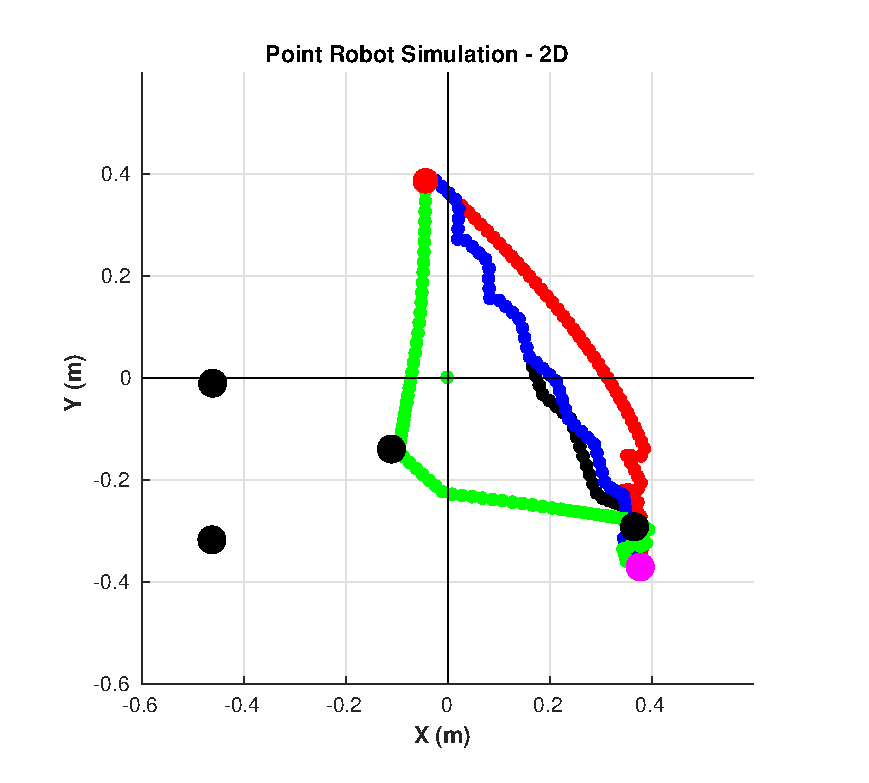
\includegraphics[width= 0.8\hsize, height=0.43\vsize]{./figures/WS_SIM.eps}
	\vspace{-0.35cm}
	\caption{Example of point-like robot simulation in $\mathbb{R}^2$. The goals are represented in black, the initial robot position in red and the human's intended goal in magenta. The different colored trajectories correspond to different mode switching schemes. Potential-based (Black), Entropy-based (Red), KL Divergence-based (Blue) and Heuristic-based (Green).} 
	\label{fig:ws_sim}
\end{figure}
 \begin{figure}[t!]
	\centering
	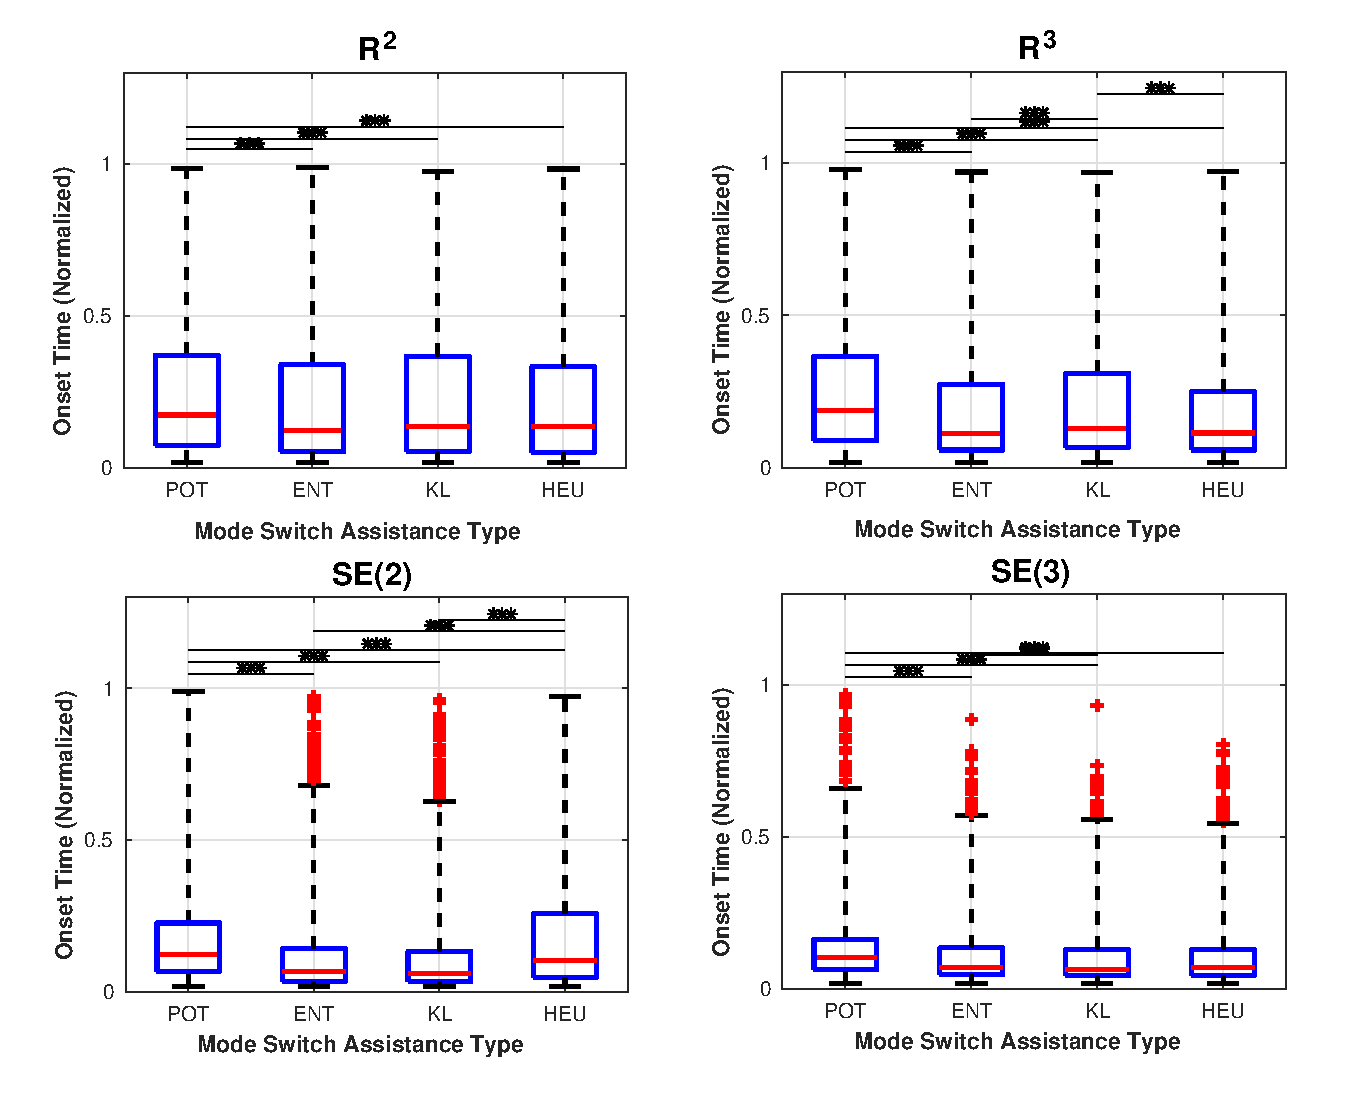
\includegraphics[width= 1.\hsize, height=0.6\vsize]{./figures/initial_alpha.eps}
	\vspace{-0.75cm}
	\caption{Group differences for initial onset of assistance for different simulation scenarios. Box plots show the median and the quartiles.} 
	\label{fig:initial_alpha}
\end{figure}



\subsection{MICO Robot Simulation Setup}
We also evaluated our system in a real robot simulation environment (MICO robotic arm from Kinova Robotics). The end effector of the robot lives in $\mathbb{SE}(3)$; however, the physical constraints of the robot make the kinematics highly nonlinear compared to a point robot in $\mathbb{SE}(3)$. We evaluated the system on two reaching tasks: 1) Four goals with same orientation and 2) five goals with different orientations. Two mode switching schemes were tested: KL divergence based disambiguation and the maximum potential based mode switching. For every trial, the robot autonomy was generated using a potential field as described in Section~\ref{sssec:autonomy}. The control mapping used for the simulations corresponded to that of a 1D discrete switch-based headarray.
Furthermore, a \textit{sparsity} factor was added to the simulated human control command $\boldsymbol{u^{sim}_h}$ to capture variability in command timing exhibited by humans. Ths sparsity factor captured the \textit{idle time} users had during task execution when teleoperating the robot. The sparsity was empirically set to be between 20-80\% as informed by the analysis of teleoperation data from previous experiments conducted in our lab. 


\section{Results}\label{sec:results}

In this section we present the results from the simulation studies conducted on point-like robots in different spaces. One way analysis of variance was performed using Kruskal-Wallis test and post-hoc analysis between groups was conducted using a multiple comparison test that used Tukey's HSD criterion. All analysis was performed in MATLAB. In all the data plots, (*) indicates $p < 0.05$, (**) indicates $p < 0.01$ and (***) indicates $p < 0.001$.
\subsection{Initial Onset of Assistance}

Kruskal-Wallis test reveals that the group ranks are different for all simulation scenarios. Post-hoc analysis also reveals statistically significant differences between the baseline mode switch assistance scheme and at least one of the disambiguation schemes for all simulation scenarios (Figure~\ref{fig:initial_alpha}). This shows that when the disambiguation scheme is used, the system is able to provide assistance \textit{earlier} during task execution. This is likely due to the fact that with disambiguation the system is able to elicit more informative control commands from the user and narrow down its prediction to the correct goal quicker during task execution. As a result, the confidence in the prediction becomes higher and the robot assistance is triggered earlier during a trial. 

\subsection{Amount of Total Assistance}
%\vspace*{-0.7cm}
\begin{figure}[t]
	\centering
	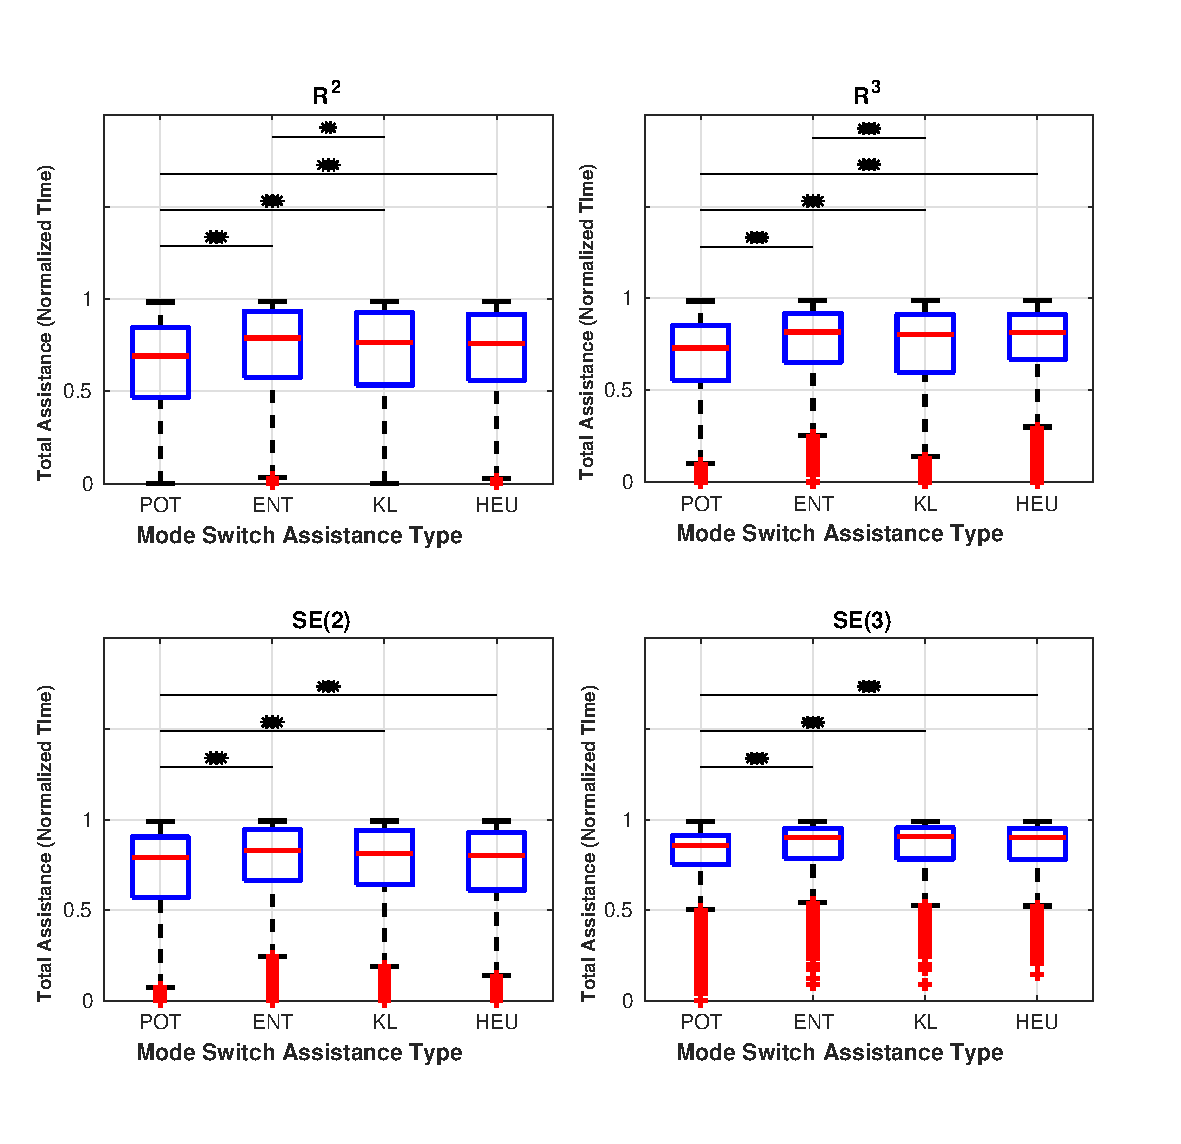
\includegraphics[width= 1.\hsize, height=0.6\vsize]{./figures/total_assistance.eps}
	\vspace{-0.8cm}
	\caption{Group differences for total amount of assistance for different simulation scenarios. Box plots show the median and the quartiles.} 
	\label{fig:total_assistance}
\end{figure}
For all simulation scenarios, Figure~\ref{fig:total_assistance} shows a statistically significant increase in the total amount of assistance when disambiguation schemes are active compared to the baseline. This is possibly because disambiguation modes help to \textit{reveal} the intent more clearly \textit{to} the robot. As a result the overall confidence in the system's prediction of intended goal increases, thereby resulting in more assistance. 
%\subsection{Number of Mode Switches}
%\begin{figure}[h]
%	\centering
%	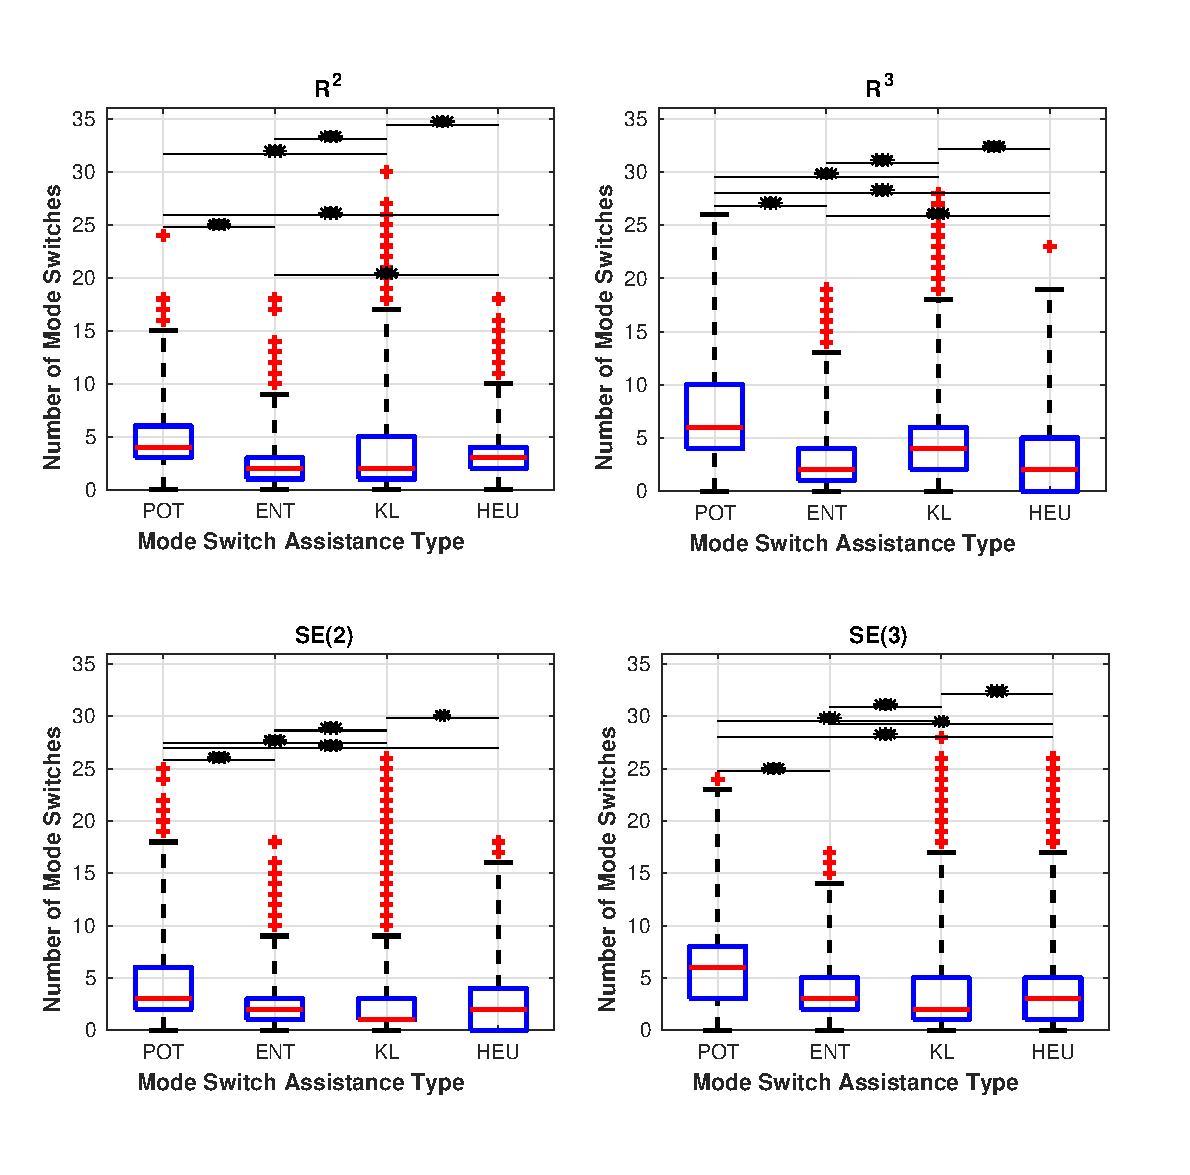
\includegraphics[width= 1.\hsize, height=0.53\vsize]{./figures/num_mode.eps}
%	\vspace{-0.35cm}
%	\caption{Group differences for total amount of assistance for different simulation scenarios. Box plots show the median and the quartiles.} 
%	\label{fig:num_mode}
%\end{figure}
%The results in Figure~\ref{fig:num_mode} shows that the number of mode switches is significantly lower for the disambiguation paradigms. Furthermore, for all simulation scenarios except $\mathbb{R}^2$, using KL divergence based disambiguation resulted in the lowest number of mode switches. 

\subsection{Inference Accuracy}
\begin{figure}[t!]
	\centering
	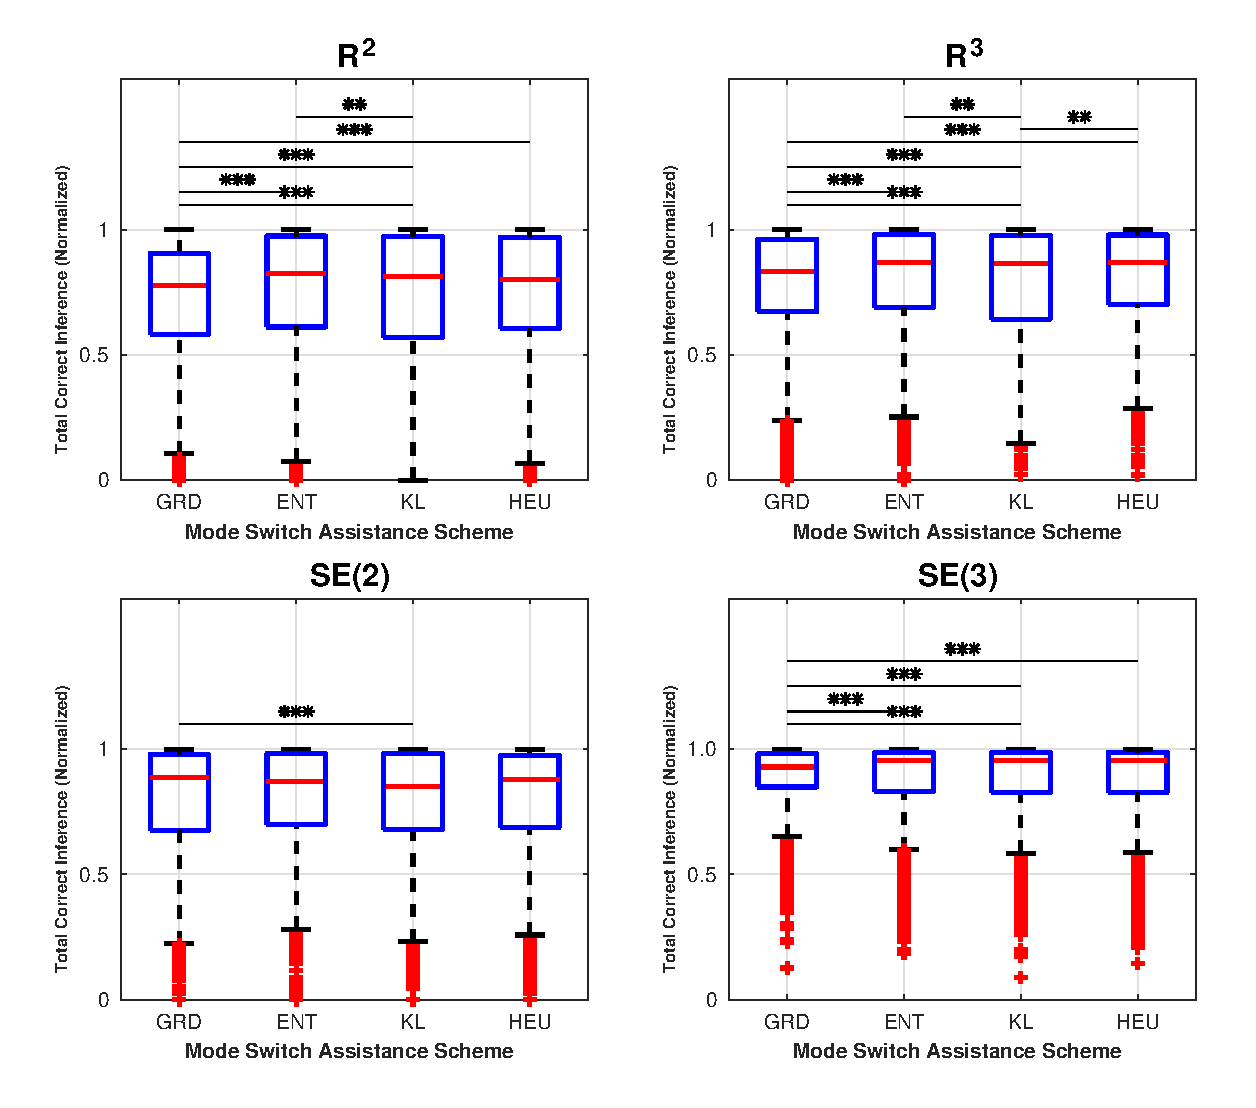
\includegraphics[width= 1.\hsize, height=0.5\vsize]{./figures/correct_inference.eps}
	\vspace{-0.75cm}
	\caption{Group differences for fractional time for correct goal inference for different simulation scenarios. Box plots show the median and the quartiles.} 
	\label{fig:correct_inference}
\end{figure}
As shown in Figure~\ref{fig:correct_inference}, for all simulation scenarios, except $\mathbb{SE}(2)$, the accuracy of intent inference was higher for the disambiguation schemes compared to the baseline. This is likely because of the fact that, disambiguating modes elicit control commands that carry more information regarding the intended goal thereby helping the system to perform accurate intent inference. 
\section{Discussion}\label{sec:discussions}
Success rate comments. 
In our experiments a single type of mode switching scheme was utilized for the entire trial. Maybe a combination of both might be useful. disambiguation in the beginning to clarify intent. once intent is clarified use greedy schemes which will ensure reaching the goal. 
Earlier assistance is important for safety critical applications.
Better tuning of the inference engine. Learning likelihood functions from data. Using DNNs for capturing the nonlinear filter in DFT. Improved kinematics model for the real robot to Real-time learning of user characteristics such as mean amplitude of control commands, how intermittent of persistent the user is issuing control commands. All of that can be incorporated into the forward projection to become as accurate as possible. 
Future work. More detailed analysis of data to expose the interactions between factors. Intent inference schemes that are amnesic might benefit from disambiguation schemes that capture informatoin gain as well as content to offset the lack of information in the probability distributions themselves. These simulated experiments have shed light on the efficacy of these systems. Full fledged human study will be done. Treating this as a mode-scheduling problem?
Explore second order metrics to capture rate of change of information. Fisher information. 


\section{Conclusion}\label{sec:conclusions}


\section*{Acknowledgments}
Funding source omitted for review. 
%% Use plainnat to work nicely with natbib. 
\balance
\bibliographystyle{plainnat}
\bibliography{references}

\end{document}


